\documentclass[aspectratio=169]{beamer}

\usepackage{amsmath, amssymb}
\usepackage{tikz}
\usetikzlibrary{calc}

\title{2D Finite Differences: Indexing, Vectorization, and Sparsity}
\subtitle{6$\times$4 grid, 5-point stencil, interior unknowns, and matrix pattern}
%\author{Mike Gosz}
\date{}

\begin{document}

%------------------------------------------------------------
\begin{frame}
  \titlepage
\end{frame}

%------------------------------------------------------------
\begin{frame}{Why we number grid points}
A 2D grid field $T_{i,j}$ becomes a vector $\mathbf{T}$ so we can write a linear system
\[
\mathbf{A}\mathbf{T}=\mathbf{b}.
\]
We need:
\begin{itemize}
  \item \textbf{Local indices} $(i,j)$ for neighbors in the stencil.
  \item \textbf{A global index} to store unknowns in a 1D vector.
\end{itemize}

\vspace{0.5em}
We will use \textbf{row-major ordering} (NumPy-style):
\[
\boxed{p = i + j\,N_x.}
\]
\end{frame}

%------------------------------------------------------------
\begin{frame}{6$\times$4 grid: $(i,j)$ labels and global index $p$ (interior labeling)}
\centering

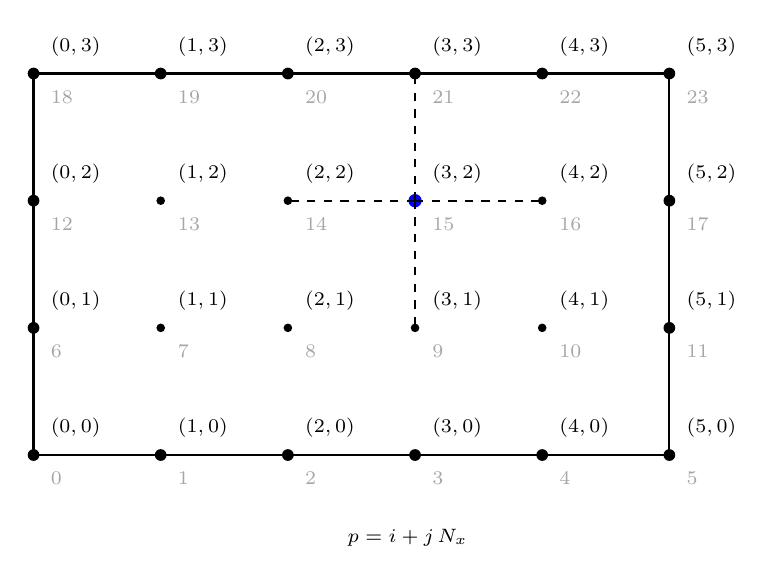
\begin{tikzpicture}[scale=1.9, every node/.style={font=\small}]
  % -----------------------------
  % USER SETTINGS
  % -----------------------------
  \def\Nx{6}   % i = 0..Nx-1
  \def\Ny{4}   % j = 0..Ny-1

  % Choose the center stencil location (must be interior)
  \def\ci{3}
  \def\cj{2}

  % Point spacing
  \def\s{0.85}

  % -----------------------------
  % STYLES
  % -----------------------------
  \tikzset{
    gp/.style={circle, fill=black, inner sep=1.1pt},
    gpb/.style={circle, fill=black, inner sep=1.5pt}, % boundary slightly larger
    gpc/.style={circle, fill=blue, inner sep=1.7pt},  % center (highlight)
    stline/.style={dashed, thick},
    labij/.style={font=\scriptsize},
    labp/.style={font=\scriptsize, text=gray!70},
  }

  % -----------------------------
  % OUTER RECTANGLE (domain)
  % -----------------------------
  \draw[thick] (0,0) rectangle ({(\Nx-1)*\s},{(\Ny-1)*\s});

  % Boundary labels
  %\node at ({(\Nx-1)*\s/2},{(\Ny-1)*\s+0.45}) {$T_T(x)$};
  %\node at ({(\Nx-1)*\s/2},{-0.52}) {$T_B(x)$};
  %\node at ({-0.68},{(\Ny-1)*\s/2}) {$T_L(y)$};
 % \node at ({(\Nx-1)*\s+0.68},{(\Ny-1)*\s/2}) {$T_R(y)$};

  % -----------------------------
  % GRID POINTS + LABELS
  % -----------------------------
  \foreach \j in {0,...,\numexpr\Ny-1\relax} {
    \foreach \i in {0,...,\numexpr\Nx-1\relax} {

      \pgfmathsetmacro{\x}{\i*\s}
      \pgfmathsetmacro{\y}{\j*\s}

      % p = i + j*Nx
      \pgfmathtruncatemacro{\p}{\i + \j*\Nx}

      % boundary test
      \pgfmathtruncatemacro{\isB}{ (\i==0) || (\i==\Nx-1) || (\j==0) || (\j==\Ny-1) }
      % center test
      \pgfmathtruncatemacro{\isC}{ (\i==\ci) && (\j==\cj) }

      \ifnum\isC=1
        \node[gpc] (P\i\j) at (\x,\y) {};
      \else
        \ifnum\isB=1
          \node[gpb] (P\i\j) at (\x,\y) {};
        \else
          \node[gp] (P\i\j) at (\x,\y) {};
        \fi
      \fi

      % Labels (i,j) above-right; p below-right
      \node[labij, anchor=south west] at (\x+0.05,\y+0.05) {$(\i,\j)$};
      \node[labp,  anchor=north west] at (\x+0.05,\y-0.05) {$\p$};
    }
  }

  % -----------------------------
  % 5-POINT STENCIL (dashed)
  % -----------------------------
  \pgfmathsetmacro{\xc}{\ci*\s}
  \pgfmathsetmacro{\yc}{\cj*\s}

  \draw[stline] (\xc,\yc) -- ({(\ci+1)*\s},\yc);
  \draw[stline] (\xc,\yc) -- ({(\ci-1)*\s},\yc);
  \draw[stline] (\xc,\yc) -- (\xc,{(\cj+1)*\s});
  \draw[stline] (\xc,\yc) -- (\xc,{(\cj-1)*\s});

  % Local stencil labels
 % \node[anchor=south] at (\xc,{(\cj+1)*\s+0.19}) {$T_{i,j+1}$};
  %\node[anchor=north] at (\xc,{(\cj-1)*\s-0.19}) {$T_{i,j-1}$};
 % \node[anchor=east]  at ({(\ci-1)*\s-0.18},\yc) {$T_{i-1,j}$};
 % \node[anchor=west]  at ({(\ci+1)*\s+0.18},\yc) {$T_{i+1,j}$};
  %\node[anchor=south] at (\xc,\yc+0.18) {$T_{i,j}$};

  % Mapping note
  \node[font=\scriptsize, align=left] at ({(1)*\s+1.65},{(0)*\s-0.55})
  {$p = i + j\,N_x$};
\end{tikzpicture}

\end{frame}

%------------------------------------------------------------
\begin{frame}{6$\times$4 grid: $(i,j)$ labels and global index $k$ (full labeling)}
\centering

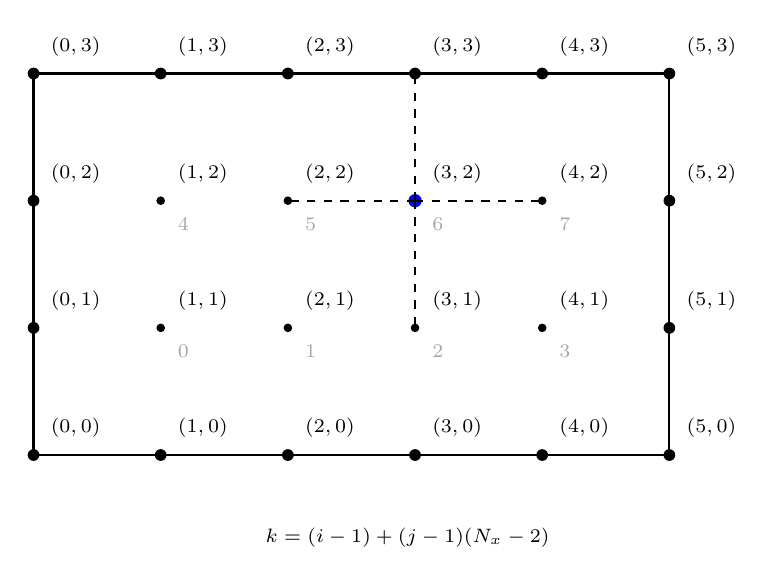
\begin{tikzpicture}[scale=1.9, every node/.style={font=\small}]
  % -----------------------------
  % USER SETTINGS
  % -----------------------------
  \def\Nx{6}   % i = 0..Nx-1
  \def\Ny{4}   % j = 0..Ny-1

  % Choose the center stencil location (must be interior)
  \def\ci{3}
  \def\cj{2}

  % Point spacing
  \def\s{0.85}

  % -----------------------------
  % STYLES
  % -----------------------------
  \tikzset{
    gp/.style={circle, fill=black, inner sep=1.1pt},
    gpb/.style={circle, fill=black, inner sep=1.5pt}, % boundary slightly larger
    gpc/.style={circle, fill=blue, inner sep=1.7pt},  % center (highlight)
    stline/.style={dashed, thick},
    labij/.style={font=\scriptsize},
    labp/.style={font=\scriptsize, text=gray!70},
  }

  % -----------------------------
  % OUTER RECTANGLE (domain)
  % -----------------------------
  \draw[thick] (0,0) rectangle ({(\Nx-1)*\s},{(\Ny-1)*\s});

  % Boundary labels
  %\node at ({(\Nx-1)*\s/2},{(\Ny-1)*\s+0.45}) {$T_T(x)$};
  %\node at ({(\Nx-1)*\s/2},{-0.52}) {$T_B(x)$};
  %\node at ({-0.68},{(\Ny-1)*\s/2}) {$T_L(y)$};
 % \node at ({(\Nx-1)*\s+0.68},{(\Ny-1)*\s/2}) {$T_R(y)$};

  % -----------------------------
  % GRID POINTS + LABELS
  % -----------------------------
  \foreach \j in {0,...,\numexpr\Ny-1\relax} {
    \foreach \i in {0,...,\numexpr\Nx-1\relax} {

      \pgfmathsetmacro{\x}{\i*\s}
      \pgfmathsetmacro{\y}{\j*\s}

      % k = (i-1) + (j-1)*(Nx-2)
      \pgfmathtruncatemacro{\p}{(\i-1) + (\j-1)*(\Nx-2)}

      % boundary test
      \pgfmathtruncatemacro{\isB}{ (\i==0) || (\i==\Nx-1) || (\j==0) || (\j==\Ny-1) }
      % center test
      \pgfmathtruncatemacro{\isC}{ (\i==\ci) && (\j==\cj) }

      \ifnum\isC=1
        \node[gpc] (P\i\j) at (\x,\y) {};
      \else
        \ifnum\isB=1
          \node[gpb] (P\i\j) at (\x,\y) {};
        \else
          \node[gp] (P\i\j) at (\x,\y) {};
        \fi
      \fi

      % Labels (i,j) above-right; p below-right
      \node[labij, anchor=south west] at (\x+0.05,\y+0.05) {$(\i,\j)$};
      \ifnum\isB=0
  \node[labp, anchor=north west] at (\x+0.05,\y-0.05) {$\p$};
\fi
    }
  }

  % -----------------------------
  % 5-POINT STENCIL (dashed)
  % -----------------------------
  \pgfmathsetmacro{\xc}{\ci*\s}
  \pgfmathsetmacro{\yc}{\cj*\s}

  \draw[stline] (\xc,\yc) -- ({(\ci+1)*\s},\yc);
  \draw[stline] (\xc,\yc) -- ({(\ci-1)*\s},\yc);
  \draw[stline] (\xc,\yc) -- (\xc,{(\cj+1)*\s});
  \draw[stline] (\xc,\yc) -- (\xc,{(\cj-1)*\s});

  % Local stencil labels
 % \node[anchor=south] at (\xc,{(\cj+1)*\s+0.19}) {$T_{i,j+1}$};
  %\node[anchor=north] at (\xc,{(\cj-1)*\s-0.19}) {$T_{i,j-1}$};
 % \node[anchor=east]  at ({(\ci-1)*\s-0.18},\yc) {$T_{i-1,j}$};
 % \node[anchor=west]  at ({(\ci+1)*\s+0.18},\yc) {$T_{i+1,j}$};
  %\node[anchor=south] at (\xc,\yc+0.18) {$T_{i,j}$};

  % Mapping note
  \node[font=\scriptsize, align=left] at ({(1)*\s+1.65},{(0)*\s-0.55})
  {$k = (i-1) + (j-1)(N_x-2)$};
\end{tikzpicture}

\end{frame}

%------------------------------------------------------------
\begin{frame}{Vector mapping and stencil offsets}
With row-major ordering ($N_x=6$):
\[
\boxed{p = i + j\,N_x} \qquad
\boxed{i = p \bmod N_x} \qquad
\boxed{j = \left\lfloor \frac{p}{N_x}\right\rfloor}
\]

For an interior node $(i,j)$ with global index $p$:
\[
\begin{aligned}
(i+1,j) &\Rightarrow p+1 \\
(i-1,j) &\Rightarrow p-1 \\
(i,j+1) &\Rightarrow p+N_x \\
(i,j-1) &\Rightarrow p-N_x
\end{aligned}
\]

So the 5-point Laplacian stencil becomes the same pattern in vector form:
\[
T_{p+1} + T_{p-1} + T_{p+N_x} + T_{p-N_x} - 4T_p
\]
\end{frame}

%------------------------------------------------------------
\begin{frame}{Sparsity pattern of $\mathbf{A}$ for interior unknowns (5-point stencil)}
\vspace{-0.25em}
\begin{itemize}
  \item Assume Dirichlet boundary values are known (moved to $\mathbf{b}$).
  \item Unknowns are the \textbf{interior} points only: $(N_x-2)\times(N_y-2)=4\times2=8$.
  \item Order unknowns in row-major order on the interior grid:
  \[k = (i-1) + (j-1)(N_x-2), \quad i=1..4,\ j=1..2.\]
\end{itemize}

\vspace{0.25em}
\centering
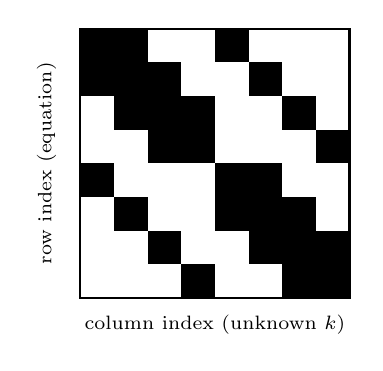
\begin{tikzpicture}[scale=0.95]
  % interior grid size
  \def\nxI{4}
  \def\nyI{2}
  \pgfmathtruncatemacro{\N}{\nxI*\nyI} % 8

  % cell size
  \def\h{0.45}

  % draw outline box
  \draw[thick] (0,0) rectangle ({\N*\h},{\N*\h});

  % draw nonzeros as filled squares
  \foreach \r in {0,...,\numexpr\N-1\relax} {
    % row index within interior row (0..nxI-1)
    \pgfmathtruncatemacro{\ri}{mod(\r,\nxI)}

    \foreach \c in {0,...,\numexpr\N-1\relax} {
      % column index within interior row (0..nxI-1)
      \pgfmathtruncatemacro{\ci}{mod(\c,\nxI)}

      % conditions for 5-point stencil coupling in row-major interior indexing
      \pgfmathtruncatemacro{\isDiag}{(\c==\r)}

      % horizontal neighbors only if not wrapping across rows
      \pgfmathtruncatemacro{\isRplus}{(\c==\r+1) && (\ri < \nxI-1)}
      \pgfmathtruncatemacro{\isRminus}{(\c==\r-1) && (\ri > 0)}

      % vertical neighbors
      \pgfmathtruncatemacro{\isUp}{(\c==\r+\nxI)}
      \pgfmathtruncatemacro{\isDown}{(\c==\r-\nxI)}

      \pgfmathtruncatemacro{\nz}{(\isDiag) || (\isRplus) || (\isRminus) || (\isUp) || (\isDown)}

      \ifnum\nz=1
        % map matrix indices to plot coordinates (row downwards)
        \pgfmathsetmacro{\x}{\c*\h}
        \pgfmathsetmacro{\y}{(\N-1-\r)*\h}
        \fill (\x,\y) rectangle ({\x+\h},{\y+\h});
      \fi
    }
  }

  % axis labels
  \node[font=\scriptsize] at ({\N*\h/2},{-0.35}) {column index (unknown $k$)};
  \node[font=\scriptsize, rotate=90] at ({-0.45},{\N*\h/2}) {row index (equation)};
\end{tikzpicture}

\vspace{0.25em}
\footnotesize
This block-banded structure comes directly from the neighbor offsets $\pm 1$ and $\pm (N_x-2)$ on the interior grid.
\end{frame}
%================================
%------------------------------------------------------------
\begin{frame}{Enforcing Dirichlet boundary conditions using slicing}
\vspace{.5em}
Suppose the temperature field is stored on a 2D grid
\[
T_{i,j}, \qquad i=0,\dots,N_x-1,\; j=0,\dots,N_y-1,
\]
with Dirichlet boundary conditions prescribed on all four edges.

\vspace{0.5em}
Using NumPy-style slicing, boundary values can be imposed \emph{without loops}:

\begin{align*}
\text{Left boundary:}   &\quad T[0, :]        = T_L(y), \\
\text{Right boundary:}  &\quad T[N_x-1, :]    = T_R(y), \\
\text{Bottom boundary:} &\quad T[:, 0]        = T_B(x), \\
\text{Top boundary:}    &\quad T[:, N_y-1]    = T_T(x).
\end{align*}

\vspace{0.5em}
Only the interior values
\[
T[1:N_x-1,\;1:N_y-1]
\]
remain unknown and are used to assemble the linear system.

\end{frame}

%------------------------------------------------------------
\begin{frame}{Takeaway}
\begin{itemize}
  \item \textbf{Local indices} $(i,j)$ express the PDE stencil naturally.
  \item A \textbf{global index} (row-major) lets us store the unknowns as a vector.
  \item The 5-point stencil becomes simple vector offsets: $\pm 1$ and $\pm N_x$ (or $\pm (N_x-2)$ for interior-only).
  \item Those offsets produce a highly \textbf{sparse, structured} matrix $\mathbf{A}$.
\end{itemize}
\end{frame}

\end{document}
